%\documentclass{report}
%\documentclass[11pt,twoside,a4paper]{report}
\documentclass[11pt,journal,compsoc]{report}[1]
\usepackage[letterpaper, margin=0.75in]{geometry}
\usepackage{lipsum}
\usepackage{epstopdf}
\usepackage{amsthm}
\PassOptionsToPackage{hyphens}{url}
\usepackage[T1]{fontenc}
\usepackage[draft]{hyperref}
\usepackage{graphicx}
\usepackage[cmex10]{amsmath}
%\usepackage{algorithmic}
%\usepackage{algorithm}
\usepackage{array}
\usepackage{mdwmath}
\usepackage{mdwtab}
\usepackage{eqparbox}
\usepackage{ucs}
\usepackage{amsmath}
\usepackage{amsfonts}
\usepackage{amssymb}
%\usepackage{graphicx}
%\usepackage{caption}
\usepackage{url}
\usepackage{multirow}
\usepackage{hhline}
\usepackage{multicol}
\usepackage{xcolor}
\usepackage{listings}
\lstset{basicstyle=\ttfamily,
  showstringspaces=false,
  commentstyle=\color{red},
  keywordstyle=\color{blue}
}


\usepackage[framemethod=tikz]{mdframed}

\definecolor{light-gray}{gray}{0.95}
\lstset{basicstyle=\scriptsize\upshape\ttfamily,tabsize=4,numbersep=10pt,language=Matlab,keywordstyle=\color{black}\bfseries}

\surroundwithmdframed[
  hidealllines=true,
  backgroundcolor=light-gray,
  innerleftmargin=10pt,
  innertopmargin=0pt,
  innerbottommargin=0pt]{lstlisting}                  

\DeclareMathOperator*{\argmin}{argmin}
\DeclareMathOperator*{\argmax}{argmax}
\newcommand*{\argminl}{\argmin\limits}
\newcommand*{\argmaxl}{\argmax\limits}
\newcommand{\Am}{\mathrm{A}}
\newcommand{\Cm}{\mathrm{C}}
\newcommand{\Gm}{\mathrm{G}}
\newcommand{\Tm}{\mathrm{T}}

\AtBeginDocument{\renewcommand{\abstractname}{}}
\renewcommand{\abstractname}{} 
\renewcommand{\baselinestretch}{1.3}

\begin{document}

\title{
%
\begin{figure}[h!]
\centerline{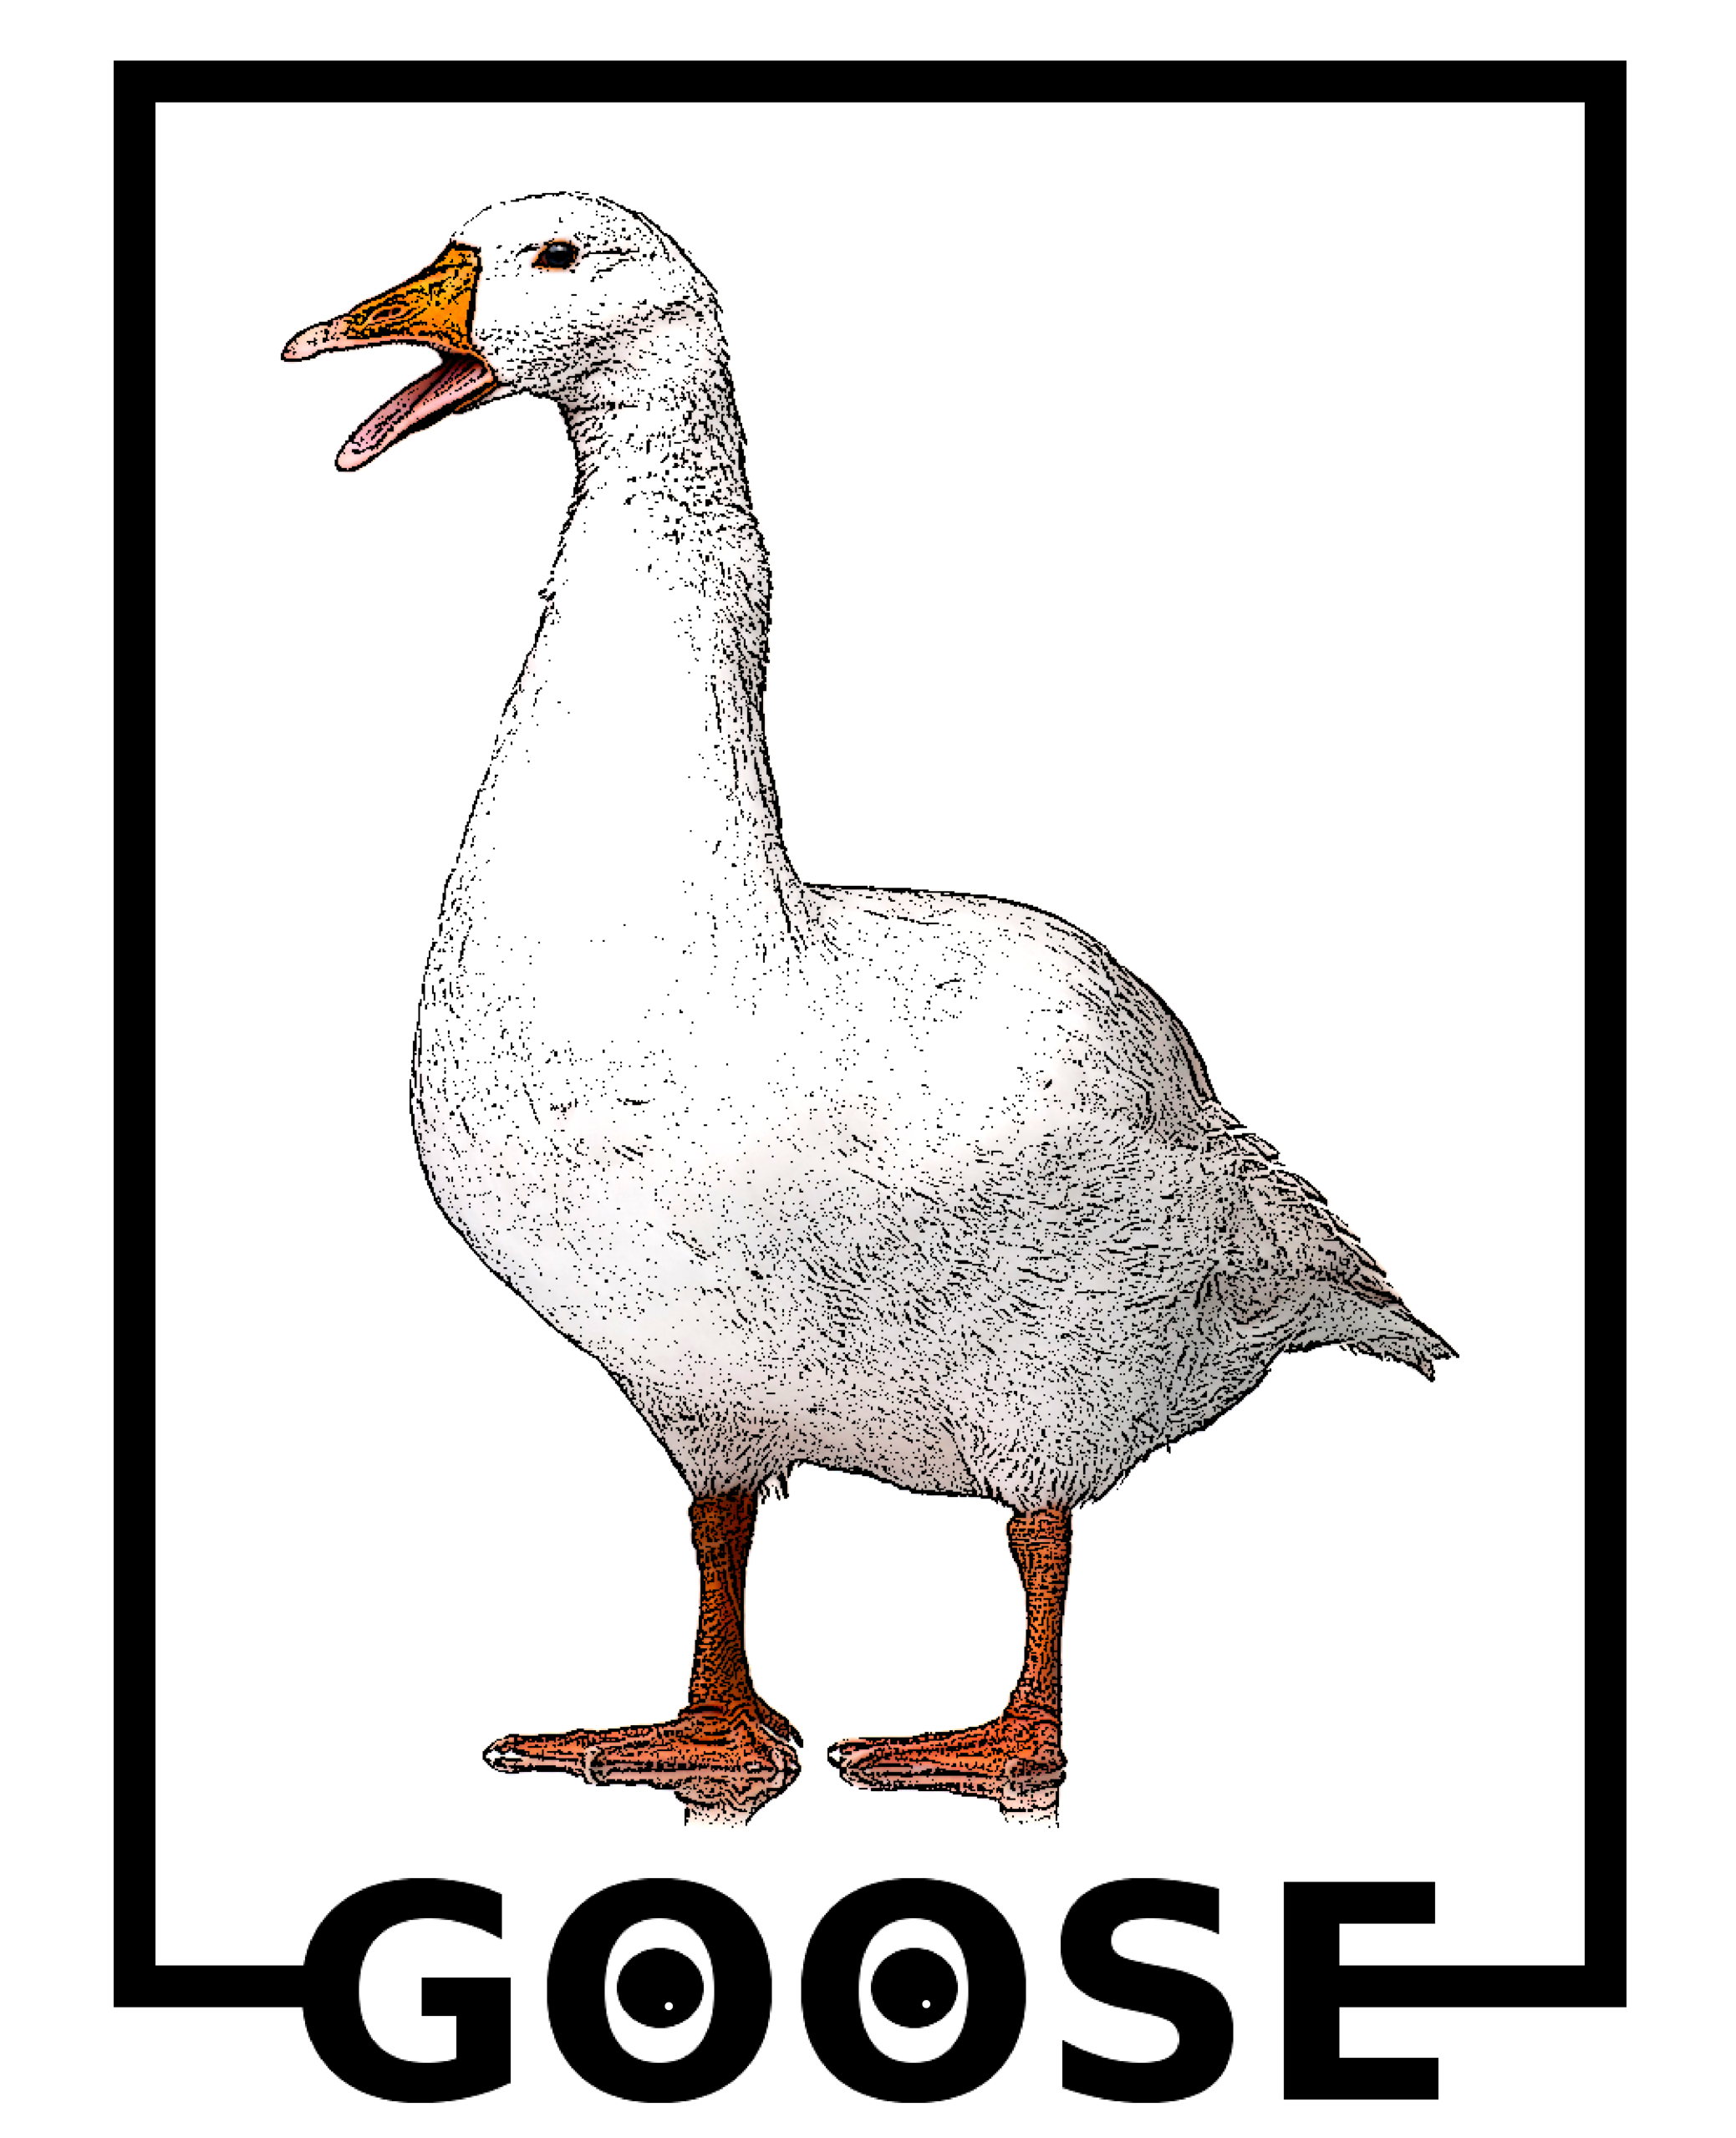
\includegraphics[width=5cm]{../imgs/logo.pdf}}
\label{logo}
\end{figure}
~\\
\textbf{A toolkit for DNA sequence\\ analysis and manipulation}
~\\~\\
\large
D. Pratas (pratas@ua.pt)\\
J. R. Almeida (joao.rafael.almeida@ua.pt)\\
A. J. Pinho (ap@ua.pt)
~\\~\\
\small
IEETA/DETI, University of Aveiro, Portugal\\
~\\
Version 1.7.17
}
\date{}
\maketitle

\tableofcontents

\def \FASTQToolsPath {sections/FASTQ_tools}
\def \FASTAToolsPath {sections/FASTA_tools}
\def \AminoAcidSequenceToolsPath {sections/Amino_acid_sequence_tools}
\def \GeneralPurposeToolsPath {sections/General_purpose_tools}

\chapter{Introduction}
\label{intro}

Recent advances in {DNA} sequencing have revolutionized the field of genomics,
making it possible for research groups to generate large amounts of sequenced
data, very rapidly and at substantially lower cost. Its storage have been
made using specific file formats, such as FASTQ and FASTA. Therefore, its
analysis and manipulation is crucial \cite{Buermans-2014a}. Several
frameworks for analysis and manipulation emerged, namely \texttt{GALAXY}
\cite{Giardine-2005a}, \texttt{GATK} \cite{DePristo-2011a}, \texttt{HTSeq}
\cite{Anders-2014a}, \texttt{MEGA} \cite{Kumar-2016a}, among others.
In the majority, these frameworks require licenses and do not provide
a low level access to the information, since they are commonly approached
by scripting or interfaces.

We describe \texttt{GOOSE}, a (free) novel toolkit for analyzing and manipulating
FASTA-FASTQ formats and sequences (DNA, amino acids, text), with many 
complementary tools. The toolkit is for Linux-based systems, built for fast 
processing. \texttt{GOOSE} supports pipes for easy integration. It includes tools 
for information display, randomizing, edition, conversion, extraction, 
searching, calculation and visualization. \texttt{GOOSE} is prepared to deal with
very large datasets, typically in the scale Gigabytes or Terabytes. 

The toolkit is a command line version, using the prefix ``goose-'' 
followed by the suffix with the respective name of the program.
\texttt{GOOSE} is implemented in \texttt{C} language and it is available, 
under GPLv3, at:
\begin{lstlisting}
https://pratas.github.io/goose
\end{lstlisting}

\section{Installation}

For \texttt{GOOSE} installation, run:
\begin{lstlisting}
git clone https://github.com/pratas/goose.git
cd goose/src/
make
\end{lstlisting}

\section{License}

The license is \textbf{GPLv3}. In resume, everyone is permitted to copy and 
distribute verbatim copies of this license document, but changing it is not 
allowed. For details on the license, consult: \url{http://www.gnu.org/licenses/gpl-3.0.html}.

\chapter{FASTQ tools}
\label{fastq}

Current available tools for FASTQ format analysis and manipulation include:
\begin{enumerate}

\item \texttt{goose-fastq2fasta}: it converts a FASTQ file format to a pseudo FASTA file.
\item \texttt{goose-fastq2mfasta}: it converts a FASTQ file format to a pseudo Multi-FASTA file.
%\item \texttt{goose-fastqclustreads}
\item \texttt{goose-FastqExcludeN}: it discards the FASTQ reads with the minimum number of "N" symbols.
\item \texttt{goose-FastqExtractQualityScores}: it extracts all the quality-scores from FASTQ reads.
\item \texttt{goose-FastqInfo}: it analyses the basic informations of FASTQ file format.
\item \texttt{goose-FastqMaximumReadSize}: it filters the FASTQ reads with the length higher than the value defined.
%\item \texttt{goose-FastqMinimumLocalQualityScoreForward}
%\item \texttt{goose-FastqMinimumLocalQualityScoreReverse}
\item \texttt{goose-FastqMinimumQualityScore}: it discards reads with average quality-score below of the defined.
\item \texttt{goose-FastqMinimumReadSize}: it filters the FASTQ reads with the length smaller than the value defined.
%\item \texttt{goose-fastqpack}
%\item \texttt{goose-fastqsimulation}
%\item \texttt{goose-FastqSplit}
%\item \texttt{goose-fastqunpack}
\item \texttt{goose-randfastqextrachars}: it substitues in the FASTQ files, the DNA sequence the outside ACGT chars by random ACGT symbols.
\item \texttt{goose-seq2fastq}: it converts a genomic sequence to pseudo FASTQ file format.
\item \texttt{goose-mutatefastq}: it creates a synthetic mutation of a FASTQ file given specific rates of mutations, deletions and additions.

%Check if theses ones are in the right chapter
%\item \texttt{goose-getunique}
%\item \texttt{goose-mfmotifcoords}
%\item \texttt{goose-period}
%\item \texttt{goose-real2binthreshold}
%\item \texttt{goose-reducematrixbythreshold}
%\item \texttt{goose-searchphash}
%\item \texttt{goose-SequenceToGroupSequence}


%Incomplete tools
%\item \texttt{goose-FastqTrimm}

\end{enumerate}

%TO DO
\section{Program goose-fastq2fasta}
The \texttt{goose-fastq2fasta} ...

For help type:
\begin{lstlisting}
./goose-fastq2fasta -h
\end{lstlisting}
In the following subsections, we explain the input and output paramters.

\subsection{Input parameters}

The \texttt{goose-fastq2fasta} program needs ...
The attribution is given according to:
\begin{lstlisting}
TO DO
\end{lstlisting}

An example on such an input file is:
\begin{lstlisting}
TO DO
\end{lstlisting}

\subsection{Output}
The output of the \texttt{goose-fastq2fasta} program ...
An example, for the input, is:
\begin{lstlisting}
TO DO
\end{lstlisting}

\section{Program goose-fastq2mfasta}
The \texttt{goose-fastq2mfasta} ...

For help type:
\begin{lstlisting}
./goose-fastq2mfasta -h
\end{lstlisting}
In the following subsections, we explain the input and output paramters.

\subsection*{Input parameters}

The \texttt{goose-fastq2mfasta} program needs ...
The attribution is given according to:
\begin{lstlisting}
TO DO
\end{lstlisting}

An example on such an input file is:
\begin{lstlisting}
TO DO
\end{lstlisting}

\subsection*{Output}
The output of the \texttt{goose-fastq2mfasta} program ...
An example, for the input, is:
\begin{lstlisting}
TO DO
\end{lstlisting}

%\section{Program goose-fastqclustreads}
The \texttt{goose-fastqclustreads} ...

For help type:
\begin{lstlisting}
./goose-fastqclustreads -h
\end{lstlisting}
In the following subsections, we explain the input and output paramters.

\subsection*{Input parameters}

The \texttt{goose-fastqclustreads} program needs ...
The attribution is given according to:
\begin{lstlisting}
TO DO
\end{lstlisting}

An example on such an input file is:
\begin{lstlisting}
TO DO
\end{lstlisting}

\subsection*{Output}
The output of the \texttt{goose-fastqclustreads} program ...
An example, for the input, is:
\begin{lstlisting}
TO DO
\end{lstlisting}

\section{Program goose-FastqExcludeN}
The \texttt{goose-FastqExcludeN} discards the FASTQ reads with the minimum number of ''N'' symbols. Also, if present, it will erase the second header (after +).\\
For help type:
\begin{lstlisting}
./goose-FastqExcludeN -h
\end{lstlisting}
In the following subsections, we explain the input and output paramters.

\subsection*{Input parameters}

The \texttt{goose-FastqExcludeN} program needs two streams for the computation,
namely the input and output standard. The input stream is a FASTQ file.\\
The attribution is given according to:
\begin{lstlisting}
Usage: ./goose-FastqExcludeN [options] [[--] args]
   or: ./goose-FastqExcludeN [options]

It discards the FASTQ reads with the minimum number of ''N'' symbols.If present,
it will erase the second header (after +).

    -h, --help            show this help message and exit

Basic options
    -m, --max=<int>       The maximum of of "N" symbols in the read
    < input.fastq         Input FASTQ file format (stdin)
    > output              Output read information (stdout)

Example: ./goose-FastqExcludeN < input.fastq > output

Output example :
<FASTQ filtered reads>
Total reads    : value
Filtered reads : value
\end{lstlisting}
An example on such an input file is:
\begin{lstlisting}
@SRR001666.1 071112_SLXA-EAS1_s_7:5:1:817:345 length=72
GNNTGATGGCCGCTGCCGATGGCGNANAATCCCACCAANATACCCTTAACAACTTAAGGGTTNTCAAATAGA
+SRR001666.1 071112_SLXA-EAS1_s_7:5:1:817:345 length=72
IIIIIIIIIIIIIIIIIIIIIIIIIIIIII9IG9ICIIIIIIIIIIIIIIIIIIIIDIIIIIII>IIIIII/
@SRR001666.2 071112_SLXA-EAS1_s_7:5:1:801:338 length=72
NTTCAGGGATACGACGNTTGTATTTTAAGAATCTGNAGCAGAAGTCGATGATAATACGCGNCGTTTTATCAN
+SRR001666.2 071112_SLXA-EAS1_s_7:5:1:801:338 length=72
IIIIIIIIIIIIIIIIIIIIIIIIIIIIIIII6IBIIIIIIIIIIIIIIIIIIIIIIIGII>IIIII-I)8I
\end{lstlisting}

\subsection*{Output}
The output of the \texttt{goose-FastqExcludeN} program is a set of all the filtered FASTQ reads, followed by the execution report.\\
Using the max value as 5, an example for this input, is: 
\begin{lstlisting}
@SRR001666.2 071112_SLXA-EAS1_s_7:5:1:801:338 length=72
NTTCAGGGATACGACGNTTGTATTTTAAGAATCTGNAGCAGAAGTCGATGATAATACGCGNCGTTTTATCAN
+
IIIIIIIIIIIIIIIIIIIIIIIIIIIIIIII6IBIIIIIIIIIIIIIIIIIIIIIIIGII>IIIII-I)8I
Total reads    : 2
Filtered reads : 1
\end{lstlisting}

\section{Program goose-FastqExtractQualityScores}
The \texttt{goose-FastqExtractQualityScores} ...

For help type:
\begin{lstlisting}
./goose-FastqExtractQualityScores -h
\end{lstlisting}
In the following subsections, we explain the input and output paramters.

\subsection*{Input parameters}

The \texttt{goose-FastqExtractQualityScores} program needs ...
The attribution is given according to:
\begin{lstlisting}
TO DO
\end{lstlisting}

An example on such an input file is:
\begin{lstlisting}
TO DO
\end{lstlisting}

\subsection*{Output}
The output of the \texttt{goose-FastqExtractQualityScores} program ...
An example, for the input, is:
\begin{lstlisting}
TO DO
\end{lstlisting}

\section{Program goose-FastqInfo}
The \texttt{goose-FastqInfo} analyses the basic informations of FASTQ file format.

For help type:
\begin{lstlisting}
./goose-FastqInfo -h
\end{lstlisting}
In the following subsections, we explain the input and output paramters.

\subsection*{Input parameters}

The \texttt{goose-FastqInfo} program needs two streams for the computation,
namely the input and output standard. The input stream is a FASTQ file.\\
The attribution is given according to:
\begin{lstlisting}
Usage: ./goose-FastqInfo [options] [[--] args]
   or: ./goose-FastqInfo [options]

It analyses the basic informations of FASTQ file format.

    -h, --help            show this help message and exit

Basic options
    < input.fastq         Input FASTQ file format (stdin)
    > output              Output read information (stdout)

Example: ./goose-FastqInfo < input.fastq > output

Output example :
Total reads     : value
Max read length : value
Min read length : value
Min QS value    : value
Max QS value    : value
QS range        : value
\end{lstlisting}
An example on such an input file is:
\begin{lstlisting}
@SRR001666.1 071112_SLXA-EAS1_s_7:5:1:817:345 length=72
GGGTGATGGCCGCTGCCGATGGCGTCAAATCCCACCAAGTTACCCTTAACAACTTAAGGGTTTTCAAATAGA
+SRR001666.1 071112_SLXA-EAS1_s_7:5:1:817:345 length=72
IIIIIIIIIIIIIIIIIIIIIIIIIIIIII9IG9ICIIIIIIIIIIIIIIIIIIIIDIIIIIII>IIIIII/
@SRR001666.2 071112_SLXA-EAS1_s_7:5:1:801:338 length=72
GTTCAGGGATACGACGTTTGTATTTTAAGAATCTGAAGCAGAAGTCGATGATAATACGCGTCGTTTTATCAT
+SRR001666.2 071112_SLXA-EAS1_s_7:5:1:801:338 length=72
IIIIIIIIIIIIIIIIIIIIIIIIIIIIIIII6IBIIIIIIIIIIIIIIIIIIIIIIIGII>IIIII-I)8I
\end{lstlisting}

\subsection*{Output}
The output of the \texttt{goose-FastqInfo} program is a set of informations related with the file readed. \\
An example, for the input, is:
\begin{lstlisting}
Total reads     : 2
Max read length : 72
Min read length : 72
Min QS value    : 41
Max QS value    : 73
QS range        : 33
\end{lstlisting}

\section{Program goose-FastqMaximumReadSize}
The \texttt{goose-FastqMaximumReadSize} filters the FASTQ reads with the length higher than the value defined.\\
For help type:
\begin{lstlisting}
./goose-FastqMaximumReadSize -h
\end{lstlisting}
In the following subsections, we explain the input and output paramters.

\subsection*{Input parameters}

The \texttt{goose-FastqMaximumReadSize} program needs two streams for the computation,
namely the input and output standard. The input stream is a FASTQ file.\\
The attribution is given according to:
\begin{lstlisting}
Usage: ./goose-FastqMaximumReadSize [options] [[--] args]
   or: ./goose-FastqMaximumReadSize [options]

It filters the FASTQ reads with the length higher than the value defined. 
If present, it will erase the second header (after +).

    -h, --help            show this help message and exit

Basic options
    -s, --size=<int>      The maximum read length
    < input.fastq         Input FASTQ file format (stdin)
    > output              Output read information (stdout)

Example: ./goose-FastqMaximumReadSize < input.fastq > output

Output example :
<FASTQ non-filtered reads>
Total reads    : value
Filtered reads : value
\end{lstlisting}
An example on such an input file is:
\begin{lstlisting}
@SRR001666.1 071112_SLXA-EAS1_s_7:5:1:817:345 length=60
GGGTGATGGCCGCTGCCGATGGCGTCAAATCCCACCAAGTTACCCTTAACAACTTAAGGG
+SRR001666.1 071112_SLXA-EAS1_s_7:5:1:817:345 length=60
IIIIIIIIIIIIIIIIIIIIIIIIIIIIII9IG9ICIIIIIIIIIIIIIIIIIIIIDIII
@SRR001666.2 071112_SLXA-EAS1_s_7:5:1:801:338 length=72
GTTCAGGGATACGACGTTTGTATTTTAAGAATCTGAAGCAGAAGTCGATGATAATACGCGTCGTTTTATCAT
+SRR001666.2 071112_SLXA-EAS1_s_7:5:1:801:338 length=72
IIIIIIIIIIIIIIIIIIIIIIIIIIIIIIII6IBIIIIIIIIIIIIIIIIIIIIIIIGII>IIIII-I)8I
\end{lstlisting}

\subsection*{Output}
The output of the \texttt{goose-FastqMaximumReadSize} program is a set of all the filtered FASTQ reads, followed by the execution report.\\
Using the size value as 60, an example for this input, is: 
\begin{lstlisting}
@SRR001666.1 071112_SLXA-EAS1_s_7:5:1:817:345 length=60
GGGTGATGGCCGCTGCCGATGGCGTCAAATCCCACCAAGTTACCCTTAACAACTTAAGGG
+
IIIIIIIIIIIIIIIIIIIIIIIIIIIIII9IG9ICIIIIIIIIIIIIIIIIIIIIDIII
Total reads    : 2
Filtered reads : 1
\end{lstlisting}

%\section{Program goose-FastqMinimumLocalQualityScoreForward}
The \texttt{goose-FastqMinimumLocalQualityScoreForward} ...

For help type:
\begin{lstlisting}
./goose-FastqMinimumLocalQualityScoreForward -h
\end{lstlisting}
In the following subsections, we explain the input and output paramters.

\subsection{Input parameters}

The \texttt{goose-FastqMinimumLocalQualityScoreForward} program needs ...
The attribution is given according to:
\begin{lstlisting}
TO DO
\end{lstlisting}

An example on such an input file is:
\begin{lstlisting}
TO DO
\end{lstlisting}

\subsection{Output}
The output of the \texttt{goose-FastqMinimumLocalQualityScoreForward} program ...
An example, for the input, is:
\begin{lstlisting}
TO DO
\end{lstlisting}

%\section{Program goose-FastqMinimumLocalQualityScoreReverse}
The \texttt{goose-FastqMinimumLocalQualityScoreReverse} ...

For help type:
\begin{lstlisting}
./goose-FastqMinimumLocalQualityScoreReverse -h
\end{lstlisting}
In the following subsections, we explain the input and output paramters.

\subsection*{Input parameters}

The \texttt{goose-FastqMinimumLocalQualityScoreReverse} program needs ...
The attribution is given according to:
\begin{lstlisting}
TO DO
\end{lstlisting}

An example on such an input file is:
\begin{lstlisting}
TO DO
\end{lstlisting}

\subsection*{Output}
The output of the \texttt{goose-FastqMinimumLocalQualityScoreReverse} program ...
An example, for the input, is:
\begin{lstlisting}
TO DO
\end{lstlisting}

\section{Program goose-FastqMinimumQualityScore}
The \texttt{goose-FastqMinimumQualityScore} discards reads with average quality-score below of the defined.\\
For help type:
\begin{lstlisting}
./goose-FastqMinimumQualityScore -h
\end{lstlisting}
In the following subsections, we explain the input and output paramters.

\subsection*{Input parameters}

The \texttt{goose-FastqMinimumQualityScore} program needs two streams for the computation,
namely the input and output standard. The input stream is a FASTQ file.\\
The attribution is given according to:
\begin{lstlisting}
Usage: ./goose-FastqMinimumQualityScore [options] [[--] args]
   or: ./goose-FastqMinimumQualityScore [options]

It discards reads with average quality-score below value.

    -h, --help            show this help message and exit

Basic options
    -m, --min=<int>       The minimum average quality-score (Value 25 or 30 is commonly used)
    < input.fastq         Input FASTQ file format (stdin)
    > output              Output read information (stdout)

Example: ./goose-FastqMinimumQualityScore < input.fastq > output

Output example :
<FASTQ non-filtered reads>
Total reads    : value
Filtered reads : value
\end{lstlisting}
An example on such an input file is:
\begin{lstlisting}
@SRR001666.1 071112_SLXA-EAS1_s_7:5:1:817:345 length=72
GGGTGATGGCCGCTGCCGATGGCGTCAAATCCCACCAAGTTACCCTTAACAACTTAAGGGTTTTCAAATAGA
+SRR001666.1 071112_SLXA-EAS1_s_7:5:1:817:345 length=72
IIIIIIIIIIIIIIIIIIIIIIIIIIIIII9IG9ICIIIIIIIIIIIIIIIIIIIIDIIIIIII>IIIIII/
@SRR001666.2 071112_SLXA-EAS1_s_7:5:1:801:338 length=72
GTTCAGGGATACGACGTTTGTATTTTAAGAATCTGAAGCAGAAGTCGATGATAATACGCGTCGTTTTATCAT
+SRR001666.2 071112_SLXA-EAS1_s_7:5:1:801:338 length=72
54599<>77977==6=?I6IBI::33344235521677999>>><<<@@A@BBCDGGBFFH>IIIII-I)8I
\end{lstlisting}

\subsection*{Output}
The output of the \texttt{goose-FastqMinimumQualityScore} program is a set of all the filtered FASTQ reads, followed by the execution report.\\
Using the minimum average value as 30, an example for this input, is:
\begin{lstlisting}
@SRR001666.1 071112_SLXA-EAS1_s_7:5:1:817:345 length=72
GGGTGATGGCCGCTGCCGATGGCGTCAAATCCCACCAAGTTACCCTTAACAACTTAAGGGTTTTCAAATAGA
+
IIIIIIIIIIIIIIIIIIIIIIIIIIIIII9IG9ICIIIIIIIIIIIIIIIIIIIIDIIIIIII>IIIIII/
Total reads    : 2
Filtered reads : 1
\end{lstlisting}

\section{Program goose-FastqMinimumReadSize}
The \texttt{goose-FastqMinimumReadSize} ...

For help type:
\begin{lstlisting}
./goose-FastqMinimumReadSize -h
\end{lstlisting}
In the following subsections, we explain the input and output paramters.

\subsection{Input parameters}

The \texttt{goose-FastqMinimumReadSize} program needs ...
The attribution is given according to:
\begin{lstlisting}
TO DO
\end{lstlisting}

An example on such an input file is:
\begin{lstlisting}
TO DO
\end{lstlisting}

\subsection{Output}
The output of the \texttt{goose-FastqMinimumReadSize} program ...
An example, for the input, is:
\begin{lstlisting}
TO DO
\end{lstlisting}

%\section{Program goose-fastqpack}
The \texttt{goose-fastqpack} ...

For help type:
\begin{lstlisting}
./goose-fastqpack -h
\end{lstlisting}
In the following subsections, we explain the input and output paramters.

\subsection*{Input parameters}

The \texttt{goose-fastqpack} program needs ...
The attribution is given according to:
\begin{lstlisting}
TO DO
\end{lstlisting}

An example on such an input file is:
\begin{lstlisting}
TO DO
\end{lstlisting}

\subsection*{Output}
The output of the \texttt{goose-fastqpack} program ...
An example, for the input, is:
\begin{lstlisting}
TO DO
\end{lstlisting}

%\section{Program goose-fastqsimulation}
The \texttt{goose-fastqsimulation} ...

For help type:
\begin{lstlisting}
./goose-fastqsimulation -h
\end{lstlisting}
In the following subsections, we explain the input and output paramters.

\subsection{Input parameters}

The \texttt{goose-fastqsimulation} program needs ...
The attribution is given according to:
\begin{lstlisting}
TO DO
\end{lstlisting}

An example on such an input file is:
\begin{lstlisting}
TO DO
\end{lstlisting}

\subsection{Output}
The output of the \texttt{goose-fastqsimulation} program ...
An example, for the input, is:
\begin{lstlisting}
TO DO
\end{lstlisting}

%\section{Program goose-FastqSplit}
The \texttt{goose-FastqSplit} ...

For help type:
\begin{lstlisting}
./goose-FastqSplit -h
\end{lstlisting}
In the following subsections, we explain the input and output paramters.

\subsection*{Input parameters}

The \texttt{goose-FastqSplit} program needs ...
The attribution is given according to:
\begin{lstlisting}
TO DO
\end{lstlisting}

An example on such an input file is:
\begin{lstlisting}
TO DO
\end{lstlisting}

\subsection*{Output}
The output of the \texttt{goose-FastqSplit} program ...
An example, for the input, is:
\begin{lstlisting}
TO DO
\end{lstlisting}


%\section{Program goose-fastqunpack}
The \texttt{goose-fastqunpack} ...

For help type:
\begin{lstlisting}
./goose-fastqunpack -h
\end{lstlisting}
In the following subsections, we explain the input and output paramters.

\subsection*{Input parameters}

The \texttt{goose-fastqunpack} program needs ...
The attribution is given according to:
\begin{lstlisting}
TO DO
\end{lstlisting}

An example on such an input file is:
\begin{lstlisting}
TO DO
\end{lstlisting}

\subsection*{Output}
The output of the \texttt{goose-fastqunpack} program ...
An example, for the input, is:
\begin{lstlisting}
TO DO
\end{lstlisting}

%\section{Program goose-getunique}
The \texttt{goose-getunique} ...

For help type:
\begin{lstlisting}
./goose-getunique -h
\end{lstlisting}
In the following subsections, we explain the input and output paramters.

\subsection*{Input parameters}

The \texttt{goose-getunique} program needs ...
The attribution is given according to:
\begin{lstlisting}
TO DO
\end{lstlisting}

An example on such an input file is:
\begin{lstlisting}
TO DO
\end{lstlisting}

\subsection*{Output}
The output of the \texttt{goose-getunique} program ...
An example, for the input, is:
\begin{lstlisting}
TO DO
\end{lstlisting}

%\section{Program goose-mfmotifcoords}
The \texttt{goose-mfmotifcoords} ...

For help type:
\begin{lstlisting}
./goose-mfmotifcoords -h
\end{lstlisting}
In the following subsections, we explain the input and output paramters.

\subsection*{Input parameters}

The \texttt{goose-mfmotifcoords} program needs ...
The attribution is given according to:
\begin{lstlisting}
TO DO
\end{lstlisting}

An example on such an input file is:
\begin{lstlisting}
TO DO
\end{lstlisting}

\subsection*{Output}
The output of the \texttt{goose-mfmotifcoords} program ...
An example, for the input, is:
\begin{lstlisting}
TO DO
\end{lstlisting}

\section{Program goose-mutatefastq}
The \texttt{goose-mutatefastq} ...

For help type:
\begin{lstlisting}
./goose-mutatefastq -h
\end{lstlisting}
In the following subsections, we explain the input and output paramters.

\subsection{Input parameters}

The \texttt{goose-mutatefastq} program needs ...
The attribution is given according to:
\begin{lstlisting}
TO DO
\end{lstlisting}

An example on such an input file is:
\begin{lstlisting}
TO DO
\end{lstlisting}

\subsection{Output}
The output of the \texttt{goose-mutatefastq} program ...
An example, for the input, is:
\begin{lstlisting}
TO DO
\end{lstlisting}

%\section{Program goose-period}
The \texttt{goose-period} ...

For help type:
\begin{lstlisting}
./goose-period -h
\end{lstlisting}
In the following subsections, we explain the input and output paramters.

\subsection*{Input parameters}

The \texttt{goose-period} program needs ...
The attribution is given according to:
\begin{lstlisting}
TO DO
\end{lstlisting}

An example on such an input file is:
\begin{lstlisting}
TO DO
\end{lstlisting}

\subsection*{Output}
The output of the \texttt{goose-period} program ...
An example, for the input, is:
\begin{lstlisting}
TO DO
\end{lstlisting}

\section{Program goose-randfastqextrachars}
The \texttt{goose-randfastqextrachars} ...

For help type:
\begin{lstlisting}
./goose-randfastqextrachars -h
\end{lstlisting}
In the following subsections, we explain the input and output paramters.

\subsection{Input parameters}

The \texttt{goose-randfastqextrachars} program needs ...
The attribution is given according to:
\begin{lstlisting}
TO DO
\end{lstlisting}

An example on such an input file is:
\begin{lstlisting}
TO DO
\end{lstlisting}

\subsection{Output}
The output of the \texttt{goose-randfastqextrachars} program ...
An example, for the input, is:
\begin{lstlisting}
TO DO
\end{lstlisting}

%\section{Program goose-real2binthreshold}
The \texttt{goose-real2binthreshold} ...

For help type:
\begin{lstlisting}
./goose-real2binthreshold -h
\end{lstlisting}
In the following subsections, we explain the input and output paramters.

\subsection{Input parameters}

The \texttt{goose-real2binthreshold} program needs ...
The attribution is given according to:
\begin{lstlisting}
TO DO
\end{lstlisting}

An example on such an input file is:
\begin{lstlisting}
TO DO
\end{lstlisting}

\subsection{Output}
The output of the \texttt{goose-real2binthreshold} program ...
An example, for the input, is:
\begin{lstlisting}
TO DO
\end{lstlisting}

%\section{Program goose-reducematrixbythreshold}
The \texttt{goose-reducematrixbythreshold} ...

For help type:
\begin{lstlisting}
./goose-reducematrixbythreshold -h
\end{lstlisting}
In the following subsections, we explain the input and output paramters.

\subsection{Input parameters}

The \texttt{goose-reducematrixbythreshold} program needs ...
The attribution is given according to:
\begin{lstlisting}
TO DO
\end{lstlisting}

An example on such an input file is:
\begin{lstlisting}
TO DO
\end{lstlisting}

\subsection{Output}
The output of the \texttt{goose-reducematrixbythreshold} program ...
An example, for the input, is:
\begin{lstlisting}
TO DO
\end{lstlisting}

%\section{Program goose-searchphash}
The \texttt{goose-searchphash} ...

For help type:
\begin{lstlisting}
./goose-searchphash -h
\end{lstlisting}
In the following subsections, we explain the input and output paramters.

\subsection{Input parameters}

The \texttt{goose-searchphash} program needs ...
The attribution is given according to:
\begin{lstlisting}
TO DO
\end{lstlisting}

An example on such an input file is:
\begin{lstlisting}
TO DO
\end{lstlisting}

\subsection{Output}
The output of the \texttt{goose-searchphash} program ...
An example, for the input, is:
\begin{lstlisting}
TO DO
\end{lstlisting}

\section{Program goose-seq2fastq}
The \texttt{goose-seq2fastq} ...

For help type:
\begin{lstlisting}
./goose-seq2fastq -h
\end{lstlisting}
In the following subsections, we explain the input and output paramters.

\subsection{Input parameters}

The \texttt{goose-seq2fastq} program needs ...
The attribution is given according to:
\begin{lstlisting}
TO DO
\end{lstlisting}

An example on such an input file is:
\begin{lstlisting}
TO DO
\end{lstlisting}

\subsection{Output}
The output of the \texttt{goose-seq2fastq} program ...
An example, for the input, is:
\begin{lstlisting}
TO DO
\end{lstlisting}

%\section{Program goose-SequenceToGroupSequence}
The \texttt{goose-SequenceToGroupSequence} ...

For help type:
\begin{lstlisting}
./goose-SequenceToGroupSequence -h
\end{lstlisting}
In the following subsections, we explain the input and output paramters.

\subsection{Input parameters}

The \texttt{goose-SequenceToGroupSequence} program needs ...
The attribution is given according to:
\begin{lstlisting}
TO DO
\end{lstlisting}

An example on such an input file is:
\begin{lstlisting}
TO DO
\end{lstlisting}

\subsection{Output}
The output of the \texttt{goose-SequenceToGroupSequence} program ...
An example, for the input, is:
\begin{lstlisting}
TO DO
\end{lstlisting}


%Incomplete tools
%%\section{Program goose-FastqTrimm}
The \texttt{goose-FastqTrimm} ...

For help type:
\begin{lstlisting}
./goose-FastqTrimm -h
\end{lstlisting}
In the following subsections, we explain the input and output paramters.

\subsection*{Input parameters}

The \texttt{goose-FastqTrimm} program needs ...
The attribution is given according to:
\begin{lstlisting}
TO DO
\end{lstlisting}

An example on such an input file is:
\begin{lstlisting}
TO DO
\end{lstlisting}

\subsection*{Output}
The output of the \texttt{goose-FastqTrimm} program ...
An example, for the input, is:
\begin{lstlisting}
TO DO
\end{lstlisting}

\chapter{FASTA tools}
\label{fasta}
%Write something about FASTA tools

Current available FASTA tools, for analysis and manipulation, are:
\begin{enumerate}
\item \texttt{goose-fasta2seq}: it converts a FASTA or Multi-FASTA file format to a seq.
\item \texttt{goose-fastaextract}: it extracts sequences from a FASTA file, which the range is defined by the user in the parameters.
\item \texttt{goose-fastaextractbyread}: it extracts sequences from each read in a Multi-FASTA file (splited by \textbackslash n), which the range is defined by the user in the parameters.
\item \texttt{goose-fastainfo}: it shows the readed information of a FASTA or Multi-FASTA file format.
\item \texttt{goose-mutatefasta}
\item \texttt{goose-randfastaextrachars}
\item \texttt{goose-geco}
\item \texttt{goose-gede}
\item \texttt{goose-mutatedna}
\item \texttt{goose-randseqextrachars}
\item \texttt{goose-reverse}: it reverses the order of a sequence.
\item \texttt{goose-reverselm}: it reverses the order of a large sequence. Low memory usage for large files.
\end{enumerate}

\section{Program goose-fasta2seq}
The \texttt{goose-fasta2seq} converts a FASTA or Multi-FASTA file format to a seq.\\
For help type:
\begin{lstlisting}
./goose-fasta2seq -h
\end{lstlisting}
In the following subsections, we explain the input and output paramters.

\subsection{Input parameters}

The \texttt{goose-fasta2seq} program needs two streams for the computation,
namely the input and output standard. The input stream is a FASTA or Multi-FASTA file.\\
The attribution is given according to:
\begin{lstlisting}
Usage: ./goose-fasta2seq [options] [[--] args]
   or: ./goose-fasta2seq [options]

It converts a FASTA or Multi-FASTA file format to a seq.

    -h, --help            show this help message and exit

Basic options
    < input.fasta         Input FASTA or Multi-FASTA file format (stdin)
    > output.seq          Output sequence file (stdout)

Example: ./goose-fasta2seq < input.fasta > output.seq
\end{lstlisting}
An example on such an input file is:
\begin{lstlisting}
>AB000264 |acc=AB000264|descr=Homo sapiens mRNA 
ACAAGACGGCCTCCTGCTGCTGCTGCTCTCCGGGGCCACGGCCCTGGAGGGTCCACCGCTGCCCTGCTGCCATTGTCCCC
GGCCCCACCTAAGGAAAAGCAGCCTCCTGACTTTCCTCGCTTGGGCCGAGACAGCGAGCATATGCAGGAAGCGGCAGGAA
GTGGTTTGAGTGGACCTCCGGGCCCCTCATAGGAGAGGAAGCTCGGGAGGTGGCCAGGCGGCAGGAAGCAGGCCAGTGCC
GCGAATCCGCGCGCCGGGACAGAATCTCCTGCAAAGCCCTGCAGGAACTTCTTCTGGAAGACCTTCTCCACCCCCCCAGC
TAAAACCTCACCCATGAATGCTCACGCAAGTTTAATTACAGACCTGAA
>AB000263 |acc=AB000263|descr=Homo sapiens mRNA 
ACAAGATGCCATTGTCCCCCGGCCTCCTGCTGCTGCTGCTCTCCGGGGCCACGGCCACCGCTGCCCTGCCCCTGGAGGGT
GGCCCCACCGGCCGAGACAGCGAGCATATGCAGGAAGCGGCAGGAATAAGGAAAAGCAGCCTCCTGACTTTCCTCGCTTG
GTGGTTTGAGTGGACCTCCCAGGCCAGTGCCGGGCCCCTCATAGGAGAGGAAGCTCGGGAGGTGGCCAGGCGGCAGGAAG
GCGCACCCCCCCAGCAATCCGCGCGCCGGGACAGAATGCCCTGCAGGAACTTCTTCTGGAAGACCTTCTCCTCCTGCAAA
TAAAACCTCACCCATGAATGCTCACGCAAGTTTAATTACAGACCTGAA
\end{lstlisting}

\subsection{Output}

The output of the \texttt{goose-fasta2seq} program is a group sequence. \\
An example, for the input, is:
\begin{lstlisting}
ACAAGACGGCCTCCTGCTGCTGCTGCTCTCCGGGGCCACGGCCCTGGAGGGTCCACCGCTGCCCTGCTGCCATTGTCCCC
GGCCCCACCTAAGGAAAAGCAGCCTCCTGACTTTCCTCGCTTGGGCCGAGACAGCGAGCATATGCAGGAAGCGGCAGGAA
GTGGTTTGAGTGGACCTCCGGGCCCCTCATAGGAGAGGAAGCTCGGGAGGTGGCCAGGCGGCAGGAAGCAGGCCAGTGCC
GCGAATCCGCGCGCCGGGACAGAATCTCCTGCAAAGCCCTGCAGGAACTTCTTCTGGAAGACCTTCTCCACCCCCCCAGC
TAAAACCTCACCCATGAATGCTCACGCAAGTTTAATTACAGACCTGAAACAAGATGCCATTGTCCCCCGGCCTCCTGCTG
CTGCTGCTCTCCGGGGCCACGGCCACCGCTGCCCTGCCCCTGGAGGGTGGCCCCACCGGCCGAGACAGCGAGCATATGCA
GGAAGCGGCAGGAATAAGGAAAAGCAGCCTCCTGACTTTCCTCGCTTGGTGGTTTGAGTGGACCTCCCAGGCCAGTGCCG
GGCCCCTCATAGGAGAGGAAGCTCGGGAGGTGGCCAGGCGGCAGGAAGGCGCACCCCCCCAGCAATCCGCGCGCCGGGAC
AGAATGCCCTGCAGGAACTTCTTCTGGAAGACCTTCTCCTCCTGCAAATAAAACCTCACCCATGAATGCTCACGCAAGTT
TAATTACAGACCTGAA
\end{lstlisting}

\section{Program goose-fastaextract}
The \texttt{goose-fastaextract} extracts sequences from a FASTA file, which the range is defined by the user in the parameters.\\
For help type:
\begin{lstlisting}
./goose-fastaextract -h
\end{lstlisting}
In the following subsections, we explain the input and output paramters.

\subsection{Input parameters}

The \texttt{goose-fastaextract} program needs two paramenters, which defines the begin and the end of the extraction, and two streams for the computation, namely the input and output standard. The input stream is a FASTA file.\\
The attribution is given according to:
\begin{lstlisting}
Usage: ./goose-fastaextract [options] [[--] args]
   or: ./goose-fastaextract [options]

It extracts sequences from a FASTA file.

    -h, --help            show this help message and exit

Basic options
    -i, --init=<int>      The first position to start the extraction (default 0)
    -e, --end=<int>       The last extract position (default 100)
    < input.fasta         Input FASTA or Multi-FASTA file format (stdin)
    > output.seq          Output sequence file (stdout)

Example: ./goose-fastaextract -i <init> -e <end> < input.fasta > output.seq
\end{lstlisting}
An example on such an input file is:
\begin{lstlisting}
>AB000264 |acc=AB000264|descr=Homo sapiens mRNA 
ACAAGACGGCCTCCTGCTGCTGCTGCTCTCCGGGGCCACGGCCCTGGAGGGTCCACCGCTGCCCTGCTGCCATTGTCCCC
GGCCCCACCTAAGGAAAAGCAGCCTCCTGACTTTCCTCGCTTGGGCCGAGACAGCGAGCATATGCAGGAAGCGGCAGGAA
GTGGTTTGAGTGGACCTCCGGGCCCCTCATAGGAGAGGAAGCTCGGGAGGTGGCCAGGCGGCAGGAAGCAGGCCAGTGCC
GCGAATCCGCGCGCCGGGACAGAATCTCCTGCAAAGCCCTGCAGGAACTTCTTCTGGAAGACCTTCTCCACCCCCCCAGC
TAAAACCTCACCCATGAATGCTCACGCAAGTTTAATTACAGACCTGAA
\end{lstlisting}

\subsection{Output}
The output of the \texttt{goose-fastaextract} program is a group sequence.\\
An example, using the value 0 as extraction starting point and the 50 as the end, for the provided input, is:
\begin{lstlisting}
ACAAGACGGCCTCCTGCTGCTGCTGCTCTCCGGGGCCACGGCCCTGGAGG
\end{lstlisting}
\section{Program goose-fastaextractbyread}
The \texttt{goose-fastaextractbyread} extracts sequences from a FASTA or Multi-FASTA file, which the range is defined by the user in the parameters.\\
For help type:
\begin{lstlisting}
./goose-fastaextractbyread -h
\end{lstlisting}
In the following subsections, we explain the input and output paramters.

\subsection*{Input parameters}

The \texttt{goose-fastaextractbyread} program needs two paramenters, which defines the begin and the end of the extraction, and two streams for the computation, namely the input and output standard. The input stream is a FASTA or Multi-FASTA file.\\
The attribution is given according to:
\begin{lstlisting}
Usage: ./goose-fastaextractbyread [options] [[--] args]
   or: ./goose-fastaextractbyread [options]

It extracts sequences from each read in a Multi-FASTA file (splited by \n)

    -h, --help            show this help message and exit

Basic options
    -i, --init=<int>      The first position to start the extraction (default 0)
    -e, --end=<int>       The last extract position (default 100)
    < input.fasta         Input FASTA or Multi-FASTA file format (stdin)
    > output.fasta        Output FASTA or Multi-FASTA file format (stdout)

Example: ./goose-fastaextractbyread -i <init> -e <end> < input.fasta > output.fasta
\end{lstlisting}
An example on such an input file is:
\begin{lstlisting}
>AB000264 |acc=AB000264|descr=Homo sapiens mRNA 
ACAAGACGGCCTCCTGCTGCTGCTGCTCTCCGGGGCCACGGCCCTGGAGGGTCCACCGCTGCCCTGCTGCCATTGTCCCC
GGCCCCACCTAAGGAAAAGCAGCCTCCTGACTTTCCTCGCTTGGGCCGAGACAGCGAGCATATGCAGGAAGCGGCAGGAA
GTGGTTTGAGTGGACCTCCGGGCCCCTCATAGGAGAGGAAGCTCGGGAGGTGGCCAGGCGGCAGGAAGCAGGCCAGTGCC
GCGAATCCGCGCGCCGGGACAGAATCTCCTGCAAAGCCCTGCAGGAACTTCTTCTGGAAGACCTTCTCCACCCCCCCAGC
TAAAACCTCACCCATGAATGCTCACGCAAGTTTAATTACAGACCTGAA
>AB000263 |acc=AB000263|descr=Homo sapiens mRNA 
ACAAGATGCCATTGTCCCCCGGCCTCCTGCTGCTGCTGCTCTCCGGGGCCACGGCCACCGCTGCCCTGCCCCTGGAGGGT
GGCCCCACCGGCCGAGACAGCGAGCATATGCAGGAAGCGGCAGGAATAAGGAAAAGCAGCCTCCTGACTTTCCTCGCTTG
GTGGTTTGAGTGGACCTCCCAGGCCAGTGCCGGGCCCCTCATAGGAGAGGAAGCTCGGGAGGTGGCCAGGCGGCAGGAAG
GCGCACCCCCCCAGCAATCCGCGCGCCGGGACAGAATGCCCTGCAGGAACTTCTTCTGGAAGACCTTCTCCTCCTGCAAA
TAAAACCTCACCCATGAATGCTCACGCAAGTTTAATTACAGACCTGAA
\end{lstlisting}

\subsection*{Output}
The output of the \texttt{goose-fastaextractbyread} program is FASTA or Multi-FASTA file wiht the extracted sequences.\\
An example, using the value 0 as extraction starting point and the 50 as the end, for the provided input, is:
\begin{lstlisting}
>AB000264 |acc=AB000264|descr=Homo sapiens mRNA 
ACAAGACGGCCTCCTGCTGCTGCTGCTCTCCGGGGCCACGGCCCTGGAGG
>AB000263 |acc=AB000263|descr=Homo sapiens mRNA 
ACAAGATGCCATTGTCCCCCGGCCTCCTGCTGCTGCTGCTCTCCGGGGCC
\end{lstlisting}
\section{Program goose-fastainfo}
The \texttt{goose-fastainfo} shows the readed information of a FASTA or Multi-FASTA file format.\\
For help type:
\begin{lstlisting}
./goose-fastainfo -h
\end{lstlisting}
In the following subsections, we explain the input and output paramters.

\subsection{Input parameters}

The \texttt{goose-fastainfo} program needs two streams for the computation,
namely the input and output standard. The input stream is a FASTA or Multi-FASTA file.\\
The attribution is given according to:
\begin{lstlisting}
Usage: ./goose-fastainfo [options] [[--] args]
   or: ./goose-fastainfo [options]

It shows read information of a FASTA or Multi-FASTA file format.

    -h, --help            show this help message and exit

Basic options
    < input.fasta         Input FASTA or Multi-FASTA file format (stdin)
    > output              Output read information (stdout)

Example: ./goose-fastainfo < input.fasta > output
\end{lstlisting}
An example on such an input file is:
\begin{lstlisting}
>AB000264 |acc=AB000264|descr=Homo sapiens mRNA 
ACAAGACGGCCTCCTGCTGCTGCTGCTCTCCGGGGCCACGGCCCTGGAGGGTCCACCGCTGCCCTGCTGCCATTGTCCCC
GGCCCCACCTAAGGAAAAGCAGCCTCCTGACTTTCCTCGCTTGGGCCGAGACAGCGAGCATATGCAGGAAGCGGCAGGAA
GTGGTTTGAGTGGACCTCCGGGCCCCTCATAGGAGAGGAAGCTCGGGAGGTGGCCAGGCGGCAGGAAGCAGGCCAGTGCC
GCGAATCCGCGCGCCGGGACAGAATCTCCTGCAAAGCCCTGCAGGAACTTCTTCTGGAAGACCTTCTCCACCCCCCCAGC
TAAAACCTCACCCATGAATGCTCACGCAAGTTTAATTACAGACCTGAA
>AB000263 |acc=AB000263|descr=Homo sapiens mRNA 
ACAAGATGCCATTGTCCCCCGGCCTCCTGCTGCTGCTGCTCTCCGGGGCCACGGCCACCGCTGCCCTGCCCCTGGAGGGT
GGCCCCACCGGCCGAGACAGCGAGCATATGCAGGAAGCGGCAGGAATAAGGAAAAGCAGCCTCCTGACTTTCCTCGCTTG
GTGGTTTGAGTGGACCTCCCAGGCCAGTGCCGGGCCCCTCATAGGAGAGGAAGCTCGGGAGGTGGCCAGGCGGCAGGAAG
GCGCACCCCCCCAGCAATCCGCGCGCCGGGACAGAATGCCCTGCAGGAACTTCTTCTGGAAGACCTTCTCCTCCTGCAAA
TAAAACCTCACCCATGAATGCTCACGCAAGTTTAATTACAGACCTGAA
\end{lstlisting}

\subsection{Output}
The output of the \texttt{goose-fastainfo} program is a set of informations related with the file readed. \\
An example, for the input, is:
\begin{lstlisting}
Number of reads      : 2
Number of bases      : 736
MIN of bases in read : 368
MAX of bases in read : 368
AVG of bases in read : 368.0000
\end{lstlisting} 
\section{Program goose-mutatefasta}
The \texttt{goose-mutatefasta} creates a synthetic mutation of a fasta file given specific rates of editions, deletions and additions. All these paramenters are defined by the user, and their are optional.\\
For help type:
\begin{lstlisting}
./goose-mutatefasta -h
\end{lstlisting}
In the following subsections, we explain the input and output paramters.

\subsection{Input parameters}

The \texttt{goose-mutatefasta} program needs two streams for the computation, namely the input and output standard. However, optional settings can be supplied too, such as the starting point to the random generator, and the edition, deletion and insertion rates. Also, the user can choose to use the ACGTN alphabet in the synthetic mutation. The input stream is a FASTA or Multi-FASTA File.\\
The attribution is given according to:
\begin{lstlisting}
Usage: ./goose-mutatefasta [options] [[--] args]
   or: ./goose-mutatefasta [options]

Creates a synthetic mutation of a fasta file given specific rates of editions, deletions and additions

    -h, --help                    show this help message and exit

Basic options
    < input.fasta                 Input FASTA or Multi-FASTA file format (stdin)
    > output.fasta                Output FASTA or Multi-FASTA file format (stdout)

Optional
    -s, --seed=<int>              Starting point to the random generator
    -e, --edit-rate=<dbl>         Defines the edition rate (default 0.0)
    -d, --deletion-rate=<dbl>     Defines the deletion rate (default 0.0)
    -i, --insertion-rate=<dbl>    Defines the insertion rate (default 0.0)
    -a, --ACGTN-alphabet          When active, the application uses the ACGTN alphabet

Example: ./goose-mutatefasta -s <seed> -e <edit rate> -d <deletion rate> -i <insertion rate> -a < input.fasta > output.fasta
\end{lstlisting}

An example on such an input file is:
\begin{lstlisting}
>AB000264 |acc=AB000264|descr=Homo sapiens mRNA 
ACAAGACGGCCTCCTGCTGCTGCTGCTCTCCGGGGCCACGGCCCTGGAGGGTCCACCGCTGCCCTGCTGCCATTGTCCCC
GGCCCCACCTAAGGAAAAGCAGCCTCCTGACTTTCCTCGCTTGGGCCGAGACAGCGAGCATATGCAGGAAGCGGCAGGAA
GTGGTTTGAGTGGACCTCCGGGCCCCTCATAGGAGAGGAAGCTCGGGAGGTGGCCAGGCGGCAGGAAGCAGGCCAGTGCC
GCGAATCCGCGCGCCGGGACAGAATCTCCTGCAAAGCCCTGCAGGAACTTCTTCTGGAAGACCTTCTCCACCCCCCCAGC
TAAAACCTCACCCATGAATGCTCACGCAAGTTTAATTACAGACCTGAA
>AB000263 |acc=AB000263|descr=Homo sapiens mRNA 
ACAAGATGCCATTGTCCCCCGGCCTCCTGCTGCTGCTGCTCTCCGGGGCCACGGCCACCGCTGCCCTGCCCCTGGAGGGT
GGCCCCACCGGCCGAGACAGCGAGCATATGCAGGAAGCGGCAGGAATAAGGAAAAGCAGCCTCCTGACTTTCCTCGCTTG
GTGGTTTGAGTGGACCTCCCAGGCCAGTGCCGGGCCCCTCATAGGAGAGGAAGCTCGGGAGGTGGCCAGGCGGCAGGAAG
GCGCACCCCCCCAGCAATCCGCGCGCCGGGACAGAATGCCCTGCAGGAACTTCTTCTGGAAGACCTTCTCCTCCTGCAAA
TAAAACCTCACCCATGAATGCTCACGCAAGTTTAATTACAGACCTGAA
\end{lstlisting}

\subsection{Output}
The output of the \texttt{goose-mutatefasta} program is a FASTA or Multi-FASTA file whith the synthetic mutation of input file.\\
Using the seed value as 1 and the edition rate as 0.5, an example for this input, is: 
\begin{lstlisting}
>AB000264 |acc=AB000264|descr=Homo sapiens mRNA 
ACGCAACGNATTCCTGCTGATCATANTGTNCCGCNCCCCNGCGACGGGGNCTCNCNNGCACACATNGTACCATTGTCCAC
NCTTNCANGTNANCGCTAGCAGGCTACNGTTTNTCCTCNCCTANNCCAANCNGGCGTNNNTACACTGGCACGTGCAGGCA
TNGGTCGGCNGGNNCCTCCGGNAACGGCACCGGAGACGAAGCTCGGNGGNTATACAGGTGTCANGAAACATCCCCGCGNC
GNGTGNCCNNGAANCCANAGAGTATCTCACTCACAACCCTGCGTGCACNTCTAGAGNANGACCTTACNCACCNTCCCNTT
NNGTACCACACCAATGAACGCTGCAGAAAGTCTGTTTNNAGGNGNGCA
>AB000263 |acc=AB000263|descr=Homo sapiens mRNA 
ATTTGAAGGCAANCGGNCCAGNAATNCGGNGGGTGCNGCTCNTGTNGGCTACGGNCATCGCGGCCCTGCTNTANTAAGCN
TGAACCACCGNTCGNNGCACTTAGCAATNGCGNAANCCGTCGGCACGGCGGAGACNAANCCGCTANTNNTTTCCCGCTNA
ATGGNTGTACAAGACCNACTANACCANCCTCCGTCACCACACTGGAGCGCANGATGGNNCGCTGNCTAGNAGNCNNTGAG
GCGCTCCNTCCTANAAANCCGTGGNCGAGCNCCCTATGGNAGNGTGGGGGTTTTACCGGAAGACCNTCGNGCCCTATGGG
AGCAATCANAANCTAGAAAGCTTACNGATGGTGANGAANTAGACTANG
\end{lstlisting}
%TO DO
%\section{Program goose-randfastaextrachars}
The \texttt{goose-randfastaextrachars} substitues in the DNA sequence the outside ACGT chars by random ACGT symbols. It works both in FASTA and Multi-FASTA file formats.\\
For help type:
\begin{lstlisting}
./goose-randfastaextrachars -h
\end{lstlisting}
In the following subsections, we explain the input and output paramters.

\subsection*{Input parameters}

The \texttt{goose-randfastaextrachars} program needs two streams for the computation,
namely the input and output standard. The input stream is a FASTA or Multi-FASTA file.\\
The attribution is given according to:
\begin{lstlisting}
Usage: ./goose-randfastaextrachars [options] [[--] args]
   or: ./goose-randfastaextrachars [options]

It substitues in the DNA sequence the outside ACGT chars by random ACGT symbols.
It works both in FASTA and Multi-FASTA file formats


    -h, --help            show this help message and exit

Basic options
    < input.fasta         Input FASTA or Multi-FASTA file format (stdin)
    > output.fasta        Output FASTA or Multi-FASTA file format (stdout)

Example: ./goose-randfastaextrachars < input.fasta > output.fasta
\end{lstlisting}

An example on such an input file is:
\begin{lstlisting}
to do
\end{lstlisting}

\subsection*{Output}
The output of the \texttt{goose-randfastaextrachars} program is a FASTA or Multi-FASTA file.\\
An example, for the input, is:
\begin{lstlisting}
to do
\end{lstlisting}
%\section{Program goose-geco}
The \texttt{goose-geco} ...

For help type:
\begin{lstlisting}
./goose-geco -h
\end{lstlisting}
In the following subsections, we explain the input and output paramters.

\subsection*{Input parameters}

The \texttt{goose-geco} program needs ...
The attribution is given according to:
\begin{lstlisting}
TO DO
\end{lstlisting}

An example on such an input file is:
\begin{lstlisting}
TO DO
\end{lstlisting}

\subsection*{Output}
The output of the \texttt{goose-geco} program ...
An example, for the input, is:
\begin{lstlisting}
TO DO
\end{lstlisting}
%\section{Program goose-gede}
The \texttt{goose-gede} ...

For help type:
\begin{lstlisting}
./goose-gede -h
\end{lstlisting}
In the following subsections, we explain the input and output paramters.

\subsection{Input parameters}

The \texttt{goose-gede} program needs ...
The attribution is given according to:
\begin{lstlisting}
TO DO
\end{lstlisting}

An example on such an input file is:
\begin{lstlisting}
TO DO
\end{lstlisting}

\subsection{Output}
The output of the \texttt{goose-gede} program ...
An example, for the input, is:
\begin{lstlisting}
TO DO
\end{lstlisting}
%\section{Program goose-mutatedna}
The \texttt{goose-mutatedna} ...

For help type:
\begin{lstlisting}
./goose-mutatedna -h
\end{lstlisting}
In the following subsections, we explain the input and output paramters.

\subsection*{Input parameters}

The \texttt{goose-mutatedna} program needs ...
The attribution is given according to:
\begin{lstlisting}
TO DO
\end{lstlisting}

An example on such an input file is:
\begin{lstlisting}
TO DO
\end{lstlisting}

\subsection*{Output}
The output of the \texttt{goose-mutatedna} program ...
An example, for the input, is:
\begin{lstlisting}
TO DO
\end{lstlisting}
%\section{Program goose-randseqextrachars}
The \texttt{goose-randseqextrachars} ...

For help type:
\begin{lstlisting}
./goose-randseqextrachars -h
\end{lstlisting}
In the following subsections, we explain the input and output paramters.

\subsection{Input parameters}

The \texttt{goose-randseqextrachars} program needs ...
The attribution is given according to:
\begin{lstlisting}
TO DO
\end{lstlisting}

An example on such an input file is:
\begin{lstlisting}
TO DO
\end{lstlisting}

\subsection{Output}
The output of the \texttt{goose-randseqextrachars} program ...
An example, for the input, is:
\begin{lstlisting}
TO DO
\end{lstlisting}
%\section{Program goose-reverse}
The \texttt{goose-reverse} reverses the order of a sequence file.

For help type:
\begin{lstlisting}
./goose-reverse -h
\end{lstlisting}
In the following subsections, we explain the input and output paramters.

\subsection*{Input parameters}

The \texttt{goose-reverse} program needs two streams for the computation,
namely the input and output standard. The input stream is a sequence file.\\
The attribution is given according to:
\begin{lstlisting}
Usage: ./goose-reverse [options] [[--] args]
   or: ./goose-reverse [options]

It reverses the order of a sequence file.

    -h, --help        show this help message and exit

Basic options
    < input.seq       Input sequence file (stdin)
    > output.seq      Output sequence file (stdout)

Example: ./goose-reverse < input.seq > output.seq
\end{lstlisting}
An example on such an input file is:
\begin{lstlisting}
ACAAGACGGCCTCCTGCTGCTGCTGCTCTCCGGGGCCACGGCCCTGGAGGGTCCACCGCTGCCCTGCTGCCATTGTCCCC
GGCCCCACCTAAGGAAAAGCAGCCTCCTGACTTTCCTCGCTTGGGCCGAGACAGCGAGCATATGCAGGAAGCGGCAGGAA
GTGGTTTGAGTGGACCTCCGGGCCCCTCATAGGAGAGGAAGCTCGGGAGGTGGCCAGGCGGCAGGAAGCAGGCCAGTGCC
GCGAATCCGCGCGCCGGGACAGAATCTCCTGCAAAGCCCTGCAGGAACTTCTTCTGGAAGACCTTCTCCACCCCCCCAGC
TAAAACCTCACCCATGAATGCTCACGCAAGTTTAATTACAGACCTGAAACAAGATGCCATTGTCCCCCGGCCTCCTGCTG
CTGCTGCTCTCCGGGGCCACGGCCACCGCTGCCCTGCCCCTGGAGGGTGGCCCCACCGGCCGAGACAGCGAGCATATGCA
GGAAGCGGCAGGAATAAGGAAAAGCAGCCTCCTGACTTTCCTCGCTTGGTGGTTTGAGTGGACCTCCCAGGCCAGTGCCG
GGCCCCTCATAGGAGAGGAAGCTCGGGAGGTGGCCAGGCGGCAGGAAGGCGCACCCCCCCAGCAATCCGCGCGCCGGGAC
AGAATGCCCTGCAGGAACTTCTTCTGGAAGACCTTCTCCTCCTGCAAATAAAACCTCACCCATGAATGCTCACGCAAGTT
TAATTACAGACCTGAA
\end{lstlisting}

\subsection*{Output}
The output of the \texttt{goose-reverse} program is a group sequence.\\
An example, for the input, is:
\begin{lstlisting}
AAGTCCAGACATTAATTTGAACGCACTCGTAAGTACCCACTCCAAAATAAACGTCCTCCTCTTCCAGAAGGTCTTCTTCA
AGGACGTCCCGTAAGACAGGGCCGCGCGCCTAACGACCCCCCCACGCGGAAGGACGGCGGACCGGTGGAGGGCTCGAAGG
AGAGGATACTCCCCGGGCCGTGACCGGACCCTCCAGGTGAGTTTGGTGGTTCGCTCCTTTCAGTCCTCCGACGAAAAGGA
ATAAGGACGGCGAAGGACGTATACGAGCGACAGAGCCGGCCACCCCGGTGGGAGGTCCCCGTCCCGTCGCCACCGGCACC
GGGGCCTCTCGTCGTCGTCGTCCTCCGGCCCCCTGTTACCGTAGAACAAAGTCCAGACATTAATTTGAACGCACTCGTAA
GTACCCACTCCAAAATCGACCCCCCCACCTCTTCCAGAAGGTCTTCTTCAAGGACGTCCCGAAACGTCCTCTAAGACAGG
GCCGCGCGCCTAAGCGCCGTGACCGGACGAAGGACGGCGGACCGGTGGAGGGCTCGAAGGAGAGGATACTCCCCGGGCCT
CCAGGTGAGTTTGGTGAAGGACGGCGAAGGACGTATACGAGCGACAGAGCCGGGTTCGCTCCTTTCAGTCCTCCGACGAA
AAGGAATCCACCCCGGCCCCTGTTACCGTCGTCCCGTCGCCACCTGGGAGGTCCCGGCACCGGGGCCTCTCGTCGTCGTC
GTCCTCCGGCAGAACA
\end{lstlisting}
%\section{Program goose-reverselm}
The \texttt{goose-reverselm} ...

For help type:
\begin{lstlisting}
./goose-reverselm -h
\end{lstlisting}
In the following subsections, we explain the input and output paramters.

\subsection{Input parameters}

The \texttt{goose-reverselm} program needs ...
The attribution is given according to:
\begin{lstlisting}
TO DO
\end{lstlisting}

An example on such an input file is:
\begin{lstlisting}
TO DO
\end{lstlisting}

\subsection{Output}
The output of the \texttt{goose-reverselm} program ...
An example, for the input, is:
\begin{lstlisting}
TO DO
\end{lstlisting}
\chapter{Amino acid sequence tools}
%\addcontentsline{toc}{chapter}{Sequence tools}
\label{seq}

Current available amino acid sequence tools, for analysis and manipulation, are:
\begin{enumerate}
\item \texttt{goose-AminoAcidToGroup}: it converts an amino acid sequence to a group 
sequence.
\item \texttt{goose-ProteinToPseudoDNA}: it converts an amino acid (protein) sequence to a pseudo DNA sequence.
\end{enumerate}

\section{Program goose-AminoAcidToGroup}

The \texttt{goose-AminoAcidToGroup} converts an amino acid sequence to a group 
sequence.\\
For help type:
\begin{lstlisting}
./goose-AminoAcidToGroup -h
\end{lstlisting}
In the following subsections, we explain the input and output paramters.

\subsection*{Input parameters}

The \texttt{goose-AminoAcidToGroup} program needs two streams for the computation,
namely the input and output standard. The input stream is an amino acid sequence.
The attribution is given according to:
\begin{lstlisting}
Usage: ./goose-AminoAcidToGroup [options] [[--] args]
   or: ./goose-AminoAcidToGroup [options]

It converts a amino acid sequence to a group sequence.

    -h, --help            show this help message and exit

Basic options
    < input.prot          Input amino acid sequence file (stdin)
    > output.group        Output group sequence file (stdout)

Example: ./goose-AminoAcidToGroup < input.prot > output.group
Table:
Prot	Group
R	P
H	P  Amino acids with electric charged side chains: POSITIVE
K	P
-	-
D	N
E	N  Amino acids with electric charged side chains: NEGATIVE
-	-
S	U
T	U
N	U  Amino acids with electric UNCHARGED side chains
Q	U
-	-
C	S
U	S
G	S  Special cases
P	S
-	-
A	H
V	H
I	H
L	H
M	H  Amino acids with hydrophobic side chains
F	H
Y	H
W	H
-	-
*	*  Others
X	X  Unknown
\end{lstlisting}
It can be used to group amino acids by properties, such as electric charge (positive
and negative), uncharged side chains, hydrophobic side chains and special cases.
An example on such an input file is:
\begin{lstlisting}
IPFLLKKQFALADKLVLSKLRQLLGGRIKMMPCGGAKLEPAIGLFFHAIGINIKLGYGMTETTATVSCWHDFQFNPNSIG
TLMPKAEVKIGENNEILVRGGMVMKGYYKKPEETAQAFTEDGFLKTGDAGEFDEQGNLFITDRIKELMKTSNGKYIAPQY
IESKIGKDKFIEQIAIIADAKKYVSALIVPCFDSLEEYAKQLNIKYHDRLELLKNSDILKMFE
\end{lstlisting}

\subsection*{Output}

The output of the \texttt{goose-AminoAcidToGroup} program is a group sequence.\\
An example, for the input, is:
\begin{lstlisting}
HSHHHPPUHHHHNPHHHUPHPUHHSSPHPHHSSSSHPHNSHHSHHHPHHSHUHPHSHSHUNUUHUHUSHPNHUHUSUUHS
UHHSPHNHPHSNUUNHHHPSSHHHPSHHPPSNNUHUHHUNNSHHPUSNHSNHNNUSUHHHUNPHPNHHPUUUSPHHHSUH
HNUPHSPNPHHNUHHHHHNHPPHHUHHHHSSHNUHNNHHPUHUHPHPNPHNHHPUUNHHPHHN
\end{lstlisting}

\section{Program goose-ProteinToPseudoDNA}

The \texttt{goose-ProteinToPseudoDNA} converts an amino acid (protein) sequence to a pseudo DNA sequence.\\
For help type:
\begin{lstlisting}
./goose-ProteinToPseudoDNA -h
\end{lstlisting}
In the following subsections, we explain the input and output paramters.

\subsection{Input parameters}

The \texttt{goose-ProteinToPseudoDNA} program needs two streams for the computation,
namely the input and output standard. The input stream is an amino acid sequence.
The attribution is given according to:
\begin{lstlisting}
Usage: ./goose-ProteinToPseudoDNA < in.prot > out.dna
It converts a protein sequence to a pseudo DNA sequence.
Table:
Prot  DNA
A	  GCA
C	  TGC
D	  GAC
E	  GAG
F	  TTT
G	  GGC
H	  CAT
I	  ATC
K	  AAA
L	  CTG
M	  ATG
N	  AAC
P	  CCG
Q	  CAG
R	  CGT
S     TCT
T	  ACG
V	  GTA
W	  TGG
Y	  TAC
*	  TAG
X	  GGG
\end{lstlisting}
It can be used to generate pseudo-DNA with characteristics passed by amino acid (protein) sequences. An example on such an input file is:
\begin{lstlisting}
IPFLLKKQFALADKLVLSKLRQLLGGRIKMMPCGGAKLEPAIGLFFHAIGINIKLGYGMTETTATVSCWHDFQFNPNSIG
TLMPKAEVKIGENNEILVRGGMVMKGYYKKPEETAQAFTEDGFLKTGDAGEFDEQGNLFITDRIKELMKTSNGKYIAPQY
IESKIGKDKFIEQIAIIADAKKYVSALIVPCFDSLEEYAKQLNIKYHDRLELLKNSDILKMFE
\end{lstlisting}

\subsection{Output}

The output of the \texttt{goose-ProteinToPseudoDNA} program is a DNA sequence.\\
An example, for the input, is:
\begin{lstlisting}
ATCCCGTTTCTGCTGAAAAAACAGTTTGCACTGGCAGACAAACTGGTACTGTCTAAACTGCGTCAGCTGCTGGGCGGCCG
TATCAAAATGATGCCGTGCGGCGGCGCAAAACTGGAGCCGGCAATCGGCCTGTTTTTTCATGCAATCGGCATCAACATCA
AACTGGGCTACGGCATGACGGAGACGACGGCAACGGTATCTTGCTGGCATGACTTTCAGTTTAACCCGAACTCTATCGGC
ACGCTGATGCCGAAAGCAGAGGTAAAAATCGGCGAGAACAACGAGATCCTGGTACGTGGCGGCATGGTAATGAAAGGCTA
CTACAAAAAACCGGAGGAGACGGCACAGGCATTTACGGAGGACGGCTTTCTGAAAACGGGCGACGCAGGCGAGTTTGACG
AGCAGGGCAACCTGTTTATCACGGACCGTATCAAAGAGCTGATGAAAACGTCTAACGGCAAATACATCGCACCGCAGTAC
ATCGAGTCTAAAATCGGCAAAGACAAATTTATCGAGCAGATCGCAATCATCGCAGACGCAAAAAAATACGTATCTGCACT
GATCGTACCGTGCTTTGACTCTCTGGAGGAGTACGCAAAACAGCTGAACATCAAATACCATGACCGTCTGGAGCTGCTGA
AAAACTCTGACATCCTGAAAATGTTTGAG
\end{lstlisting}


\chapter{General purpose tools}
\label{seq}

\begin{enumerate}
\item \texttt{goose-comparativemap}%: visualisation of comparative maps. It builds a image given specific patterns between two sequences.
\item \texttt{goose-BruteForceString}%: it generates, line by line, multiple combinations of strings up to a certain size.
\item \texttt{goose-char2line}%: it transforms each char into a char in each line.
\item \texttt{goose-sum}%: it adds the second column value to the first column value.
\item \texttt{goose-min}%: it finds the minimum value between two column values.
\item \texttt{goose-minus}%: it substracts the second column value to the first column value.
\item \texttt{goose-max}%: it finds the mmaximum value between two column values.
\item \texttt{goose-extract}%: it extracts a subsequence of a sequence by coordinates.
\item \texttt{goose-segment}%: it segments a sequence given a certain threshold.
\item \texttt{goose-reverse}: it reverses the order of a sequence.
\end{enumerate}

%TO DO
%\section{Program goose-comparativemap}
The \texttt{goose-comparativemap} ...

For help type:
\begin{lstlisting}
./goose-comparativemap -h
\end{lstlisting}
In the following subsections, we explain the input and output paramters.

\subsection*{Input parameters}

The \texttt{goose-comparativemap} program needs ...
The attribution is given according to:
\begin{lstlisting}
TO DO
\end{lstlisting}

An example on such an input file is:
\begin{lstlisting}
TO DO
\end{lstlisting}

\subsection*{Output}
The output of the \texttt{goose-comparativemap} program ...
An example, for the input, is:
\begin{lstlisting}
TO DO
\end{lstlisting}
%\section{Program goose-BruteForceString}
The \texttt{goose-BruteForceString} ...

For help type:
\begin{lstlisting}
./goose-BruteForceString -h
\end{lstlisting}
In the following subsections, we explain the input and output paramters.

\subsection*{Input parameters}

The \texttt{goose-BruteForceString} program needs ...
The attribution is given according to:
\begin{lstlisting}
TO DO
\end{lstlisting}

An example on such an input file is:
\begin{lstlisting}
TO DO
\end{lstlisting}

\subsection*{Output}
The output of the \texttt{goose-BruteForceString} program ...
An example, for the input, is:
\begin{lstlisting}
TO DO
\end{lstlisting}
%\section{Program goose-char2line}
The \texttt{goose-char2line} splits a sequence into lines, creating an output sequence which has a char for each line.

For help type:
\begin{lstlisting}
./goose-char2line -h
\end{lstlisting}
In the following subsections, we explain the input and output paramters.

\subsection*{Input parameters}

The \texttt{goose-char2line} program needs two streams for the computation,
namely the input and output standard. The input stream is a sequence file.\\
The attribution is given according to:
\begin{lstlisting}
Usage: ./goose-char2line [options] [[--] args]
   or: ./goose-char2line [options]

It splits a sequence into lines, creating an output sequence which has a char for each line.

    -h, --help        show this help message and exit

Basic options
    < input.seq       Input sequence file (stdin)
    > output.seq      Output sequence file (stdout)

Example: ./goose-char2line < input.seq > output.seq
\end{lstlisting}
An example on such an input file is:
\begin{lstlisting}
ACAAGACGGCCTCCTGCTGCTGCTGCTCTCCGGGGCCACGGCCCTGGAGGGTCCACCGCTGCCCTGCTGCCATTGTCCCC
GGCCCCACCTAAGGAAAAGCAGCCTCCTGACTTTCCTCGCTTGGGCCGAGACAGCGAGCATATGCAGGAAGCGGCAGGAA
GTGGTTTGAGTGGACCTCCGGGCCCCTCATAGGAGAGGAAGCTCGGGAGGTGGCCAGGCGGCAGGAAGCAGGCCAGTGCC
GCGAATCCGCGCGCCGGGACAGAATCTCCTGCAAAGCCCTGCAGGAACTTCTTCTGGAAGACCTTCTCCACCCCCCCAGC
TAAAACCTCACCCATGAATGCTCACGCAAGTTTAATTACAGACCTGAAACAAGATGCCATTGTCCCCCGGCCTCCTGCTG
CTGCTGCTCTCCGGGGCCACGGCCACCGCTGCCCTGCCCCTGGAGGGTGGCCCCACCGGCCGAGACAGCGAGCATATGCA
GGAAGCGGCAGGAATAAGGAAAAGCAGCCTCCTGACTTTCCTCGCTTGGTGGTTTGAGTGGACCTCCCAGGCCAGTGCCG
GGCCCCTCATAGGAGAGGAAGCTCGGGAGGTGGCCAGGCGGCAGGAAGGCGCACCCCCCCAGCAATCCGCGCGCCGGGAC
AGAATGCCCTGCAGGAACTTCTTCTGGAAGACCTTCTCCTCCTGCAAATAAAACCTCACCCATGAATGCTCACGCAAGTT
TAATTACAGACCTGAA
\end{lstlisting}

\subsection*{Output}
The output of the \texttt{goose-char2line} program is a group sequence splited by \textbackslash n foreach character.\\
An example, for the input, is:
\begin{lstlisting}
A
C
A
A
G
A
C
G
G
C
C
T
C
C
T
G
C
T
G
C
T
...
\end{lstlisting}
%\section{Program goose-sum}
The \texttt{goose-sum} ...

For help type:
\begin{lstlisting}
./goose-sum -h
\end{lstlisting}
In the following subsections, we explain the input and output paramters.

\subsection*{Input parameters}

The \texttt{goose-sum} program needs ...
The attribution is given according to:
\begin{lstlisting}
TO DO
\end{lstlisting}

An example on such an input file is:
\begin{lstlisting}
TO DO
\end{lstlisting}

\subsection*{Output}
The output of the \texttt{goose-sum} program ...
An example, for the input, is:
\begin{lstlisting}
TO DO
\end{lstlisting}
%\section{Program goose-min}
The \texttt{goose-min} ...

For help type:
\begin{lstlisting}
./goose-min -h
\end{lstlisting}
In the following subsections, we explain the input and output paramters.

\subsection{Input parameters}

The \texttt{goose-min} program needs ...
The attribution is given according to:
\begin{lstlisting}
TO DO
\end{lstlisting}

An example on such an input file is:
\begin{lstlisting}
TO DO
\end{lstlisting}

\subsection{Output}
The output of the \texttt{goose-min} program ...
An example, for the input, is:
\begin{lstlisting}
TO DO
\end{lstlisting}
%\section{Program goose-minus}
The \texttt{goose-minus} ...

For help type:
\begin{lstlisting}
./goose-minus -h
\end{lstlisting}
In the following subsections, we explain the input and output paramters.

\subsection*{Input parameters}

The \texttt{goose-minus} program needs ...
The attribution is given according to:
\begin{lstlisting}
TO DO
\end{lstlisting}

An example on such an input file is:
\begin{lstlisting}
TO DO
\end{lstlisting}

\subsection*{Output}
The output of the \texttt{goose-minus} program ...
An example, for the input, is:
\begin{lstlisting}
TO DO
\end{lstlisting}
%\section{Program goose-max}
The \texttt{goose-max} ...

For help type:
\begin{lstlisting}
./goose-max -h
\end{lstlisting}
In the following subsections, we explain the input and output paramters.

\subsection{Input parameters}

The \texttt{goose-max} program needs ...
The attribution is given according to:
\begin{lstlisting}
TO DO
\end{lstlisting}

An example on such an input file is:
\begin{lstlisting}
TO DO
\end{lstlisting}

\subsection{Output}
The output of the \texttt{goose-max} program ...
An example, for the input, is:
\begin{lstlisting}
TO DO
\end{lstlisting}
%\section{Program goose-extract}
The \texttt{goose-extract} ...

For help type:
\begin{lstlisting}
./goose-extract -h
\end{lstlisting}
In the following subsections, we explain the input and output paramters.

\subsection{Input parameters}

The \texttt{goose-extract} program needs ...
The attribution is given according to:
\begin{lstlisting}
TO DO
\end{lstlisting}

An example on such an input file is:
\begin{lstlisting}
TO DO
\end{lstlisting}

\subsection{Output}
The output of the \texttt{goose-extract} program ...
An example, for the input, is:
\begin{lstlisting}
TO DO
\end{lstlisting}
%\section{Program goose-segment}
The \texttt{goose-segment} ...

For help type:
\begin{lstlisting}
./goose-segment -h
\end{lstlisting}
In the following subsections, we explain the input and output paramters.

\subsection{Input parameters}

The \texttt{goose-segment} program needs ...
The attribution is given according to:
\begin{lstlisting}
TO DO
\end{lstlisting}

An example on such an input file is:
\begin{lstlisting}
TO DO
\end{lstlisting}

\subsection{Output}
The output of the \texttt{goose-segment} program ...
An example, for the input, is:
\begin{lstlisting}
TO DO
\end{lstlisting}
\section{Program goose-reverse}
The \texttt{goose-reverse} reverses the order of a sequence file.

For help type:
\begin{lstlisting}
./goose-reverse -h
\end{lstlisting}
In the following subsections, we explain the input and output paramters.

\subsection*{Input parameters}

The \texttt{goose-reverse} program needs two streams for the computation,
namely the input and output standard. The input stream is a sequence file.\\
The attribution is given according to:
\begin{lstlisting}
Usage: ./goose-reverse [options] [[--] args]
   or: ./goose-reverse [options]

It reverses the order of a sequence file.

    -h, --help        show this help message and exit

Basic options
    < input.seq       Input sequence file (stdin)
    > output.seq      Output sequence file (stdout)

Example: ./goose-reverse < input.seq > output.seq
\end{lstlisting}
An example on such an input file is:
\begin{lstlisting}
ACAAGACGGCCTCCTGCTGCTGCTGCTCTCCGGGGCCACGGCCCTGGAGGGTCCACCGCTGCCCTGCTGCCATTGTCCCC
GGCCCCACCTAAGGAAAAGCAGCCTCCTGACTTTCCTCGCTTGGGCCGAGACAGCGAGCATATGCAGGAAGCGGCAGGAA
GTGGTTTGAGTGGACCTCCGGGCCCCTCATAGGAGAGGAAGCTCGGGAGGTGGCCAGGCGGCAGGAAGCAGGCCAGTGCC
GCGAATCCGCGCGCCGGGACAGAATCTCCTGCAAAGCCCTGCAGGAACTTCTTCTGGAAGACCTTCTCCACCCCCCCAGC
TAAAACCTCACCCATGAATGCTCACGCAAGTTTAATTACAGACCTGAAACAAGATGCCATTGTCCCCCGGCCTCCTGCTG
CTGCTGCTCTCCGGGGCCACGGCCACCGCTGCCCTGCCCCTGGAGGGTGGCCCCACCGGCCGAGACAGCGAGCATATGCA
GGAAGCGGCAGGAATAAGGAAAAGCAGCCTCCTGACTTTCCTCGCTTGGTGGTTTGAGTGGACCTCCCAGGCCAGTGCCG
GGCCCCTCATAGGAGAGGAAGCTCGGGAGGTGGCCAGGCGGCAGGAAGGCGCACCCCCCCAGCAATCCGCGCGCCGGGAC
AGAATGCCCTGCAGGAACTTCTTCTGGAAGACCTTCTCCTCCTGCAAATAAAACCTCACCCATGAATGCTCACGCAAGTT
TAATTACAGACCTGAA
\end{lstlisting}

\subsection*{Output}
The output of the \texttt{goose-reverse} program is a group sequence.\\
An example, for the input, is:
\begin{lstlisting}
AAGTCCAGACATTAATTTGAACGCACTCGTAAGTACCCACTCCAAAATAAACGTCCTCCTCTTCCAGAAGGTCTTCTTCA
AGGACGTCCCGTAAGACAGGGCCGCGCGCCTAACGACCCCCCCACGCGGAAGGACGGCGGACCGGTGGAGGGCTCGAAGG
AGAGGATACTCCCCGGGCCGTGACCGGACCCTCCAGGTGAGTTTGGTGGTTCGCTCCTTTCAGTCCTCCGACGAAAAGGA
ATAAGGACGGCGAAGGACGTATACGAGCGACAGAGCCGGCCACCCCGGTGGGAGGTCCCCGTCCCGTCGCCACCGGCACC
GGGGCCTCTCGTCGTCGTCGTCCTCCGGCCCCCTGTTACCGTAGAACAAAGTCCAGACATTAATTTGAACGCACTCGTAA
GTACCCACTCCAAAATCGACCCCCCCACCTCTTCCAGAAGGTCTTCTTCAAGGACGTCCCGAAACGTCCTCTAAGACAGG
GCCGCGCGCCTAAGCGCCGTGACCGGACGAAGGACGGCGGACCGGTGGAGGGCTCGAAGGAGAGGATACTCCCCGGGCCT
CCAGGTGAGTTTGGTGAAGGACGGCGAAGGACGTATACGAGCGACAGAGCCGGGTTCGCTCCTTTCAGTCCTCCGACGAA
AAGGAATCCACCCCGGCCCCTGTTACCGTCGTCCCGTCGCCACCTGGGAGGTCCCGGCACCGGGGCCTCTCGTCGTCGTC
GTCCTCCGGCAGAACA
\end{lstlisting}


\addcontentsline{toc}{chapter}{Bibliography}
\bibliographystyle{IEEEtran}
\bibliography{defs,SPLc,SPLj,Cod,Bio,Book,Anc,Patho}

\end{document}
